\documentclass[xcolor=svgnames]{beamer}
\mode<presentation>
{
      \setbeamertemplate{footline}[page number]
      \setbeamercovered{transparent}
      \setbeamertemplate{navigation symbols}{}
      \usecolortheme[named=DarkGreen]{structure}
}

\usepackage[english]{babel}
\usepackage{times}
\usepackage{url}
\usepackage{CJKutf8}
\usepackage{graphics}
\usepackage{amsmath}
\usepackage{listings}
\lstset{breakatwhitespace,
language=C,
columns=fullflexible,
keepspaces,
breaklines,
tabsize=3,
showstringspaces=false,
extendedchars=true}


\AtBeginSubsection[]
{
    \begin{frame}<beamer>{Outline}
    \tableofcontents[currentsection,currentsubsection]
    \end{frame}
}


\begin{document}
\begin{CJK*}{UTF8}{gbsn}


\title{OS概念与Linux内核代码分析之一:进程管理}
\author{李中国}
\institute{苏州大学计算机科学与技术学院} 

\begin{frame}
\maketitle
\end{frame}

\begin{frame}{内容提要}
\tableofcontents[pausesections]
\end{frame}

\section{本部分课程简介}

\begin{frame}[fragile]
\frametitle{本课程Linux内核版本}
\begin{itemize}
\item linux kernel: 2.6.11.12 
\item 为什么使用这个版本的内核?
\item 下载地址: \url{http://www.kernel.org/pub/linux/kernel/v2.6}
\end{itemize}
\end{frame}

\begin{frame}[fragile]%{Linux内核关键数据结构:list}
\frametitle{为什么研究Linux内核代码}
\begin{itemize}
\item 了解OS的概念如何应用于实际操作系统
\item 学习顶尖高手写程序的思路与方法
\item 学习数据结构与算法如何用于解决实际问题
\item 学习大规模工程的设计与实施
\begin{itemize}
\item 2.6.x内核开发成本: \$1.14 billion USD (欧盟)
\item 最新内核开发成本: \$3.0 billion USD (Wikipedia)
\end{itemize}
\item 成为一名内核开发人员
\end{itemize}
\end{frame}

\begin{frame}[fragile]%{Linux内核关键数据结构:list}
\frametitle{Linux内核整体架构}
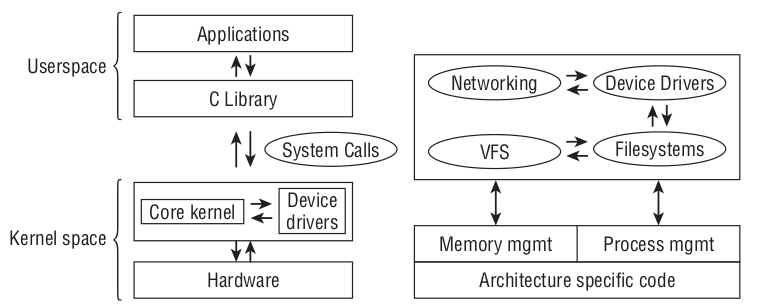
\includegraphics[width=1.0\textwidth]{kernel.png}
\end{frame}


\section{Linux内核关键数据结构}

\subsection{双向循环链表: list\_head}

\defverbatim[colored]\lstfox{
\begin{lstlisting}[tabsize=8,basicstyle=\ttfamily]
struct fox {
    unsigned long tail_length;
    unsigned long weight;
    bool     is_fantastic;
    struct fox *next;
    struct fox *prev;
};
\end{lstlisting}
}
\begin{frame}[fragile]
\frametitle{双向链表的常见实现方式}
\lstfox
\begin{block}{思考:}
这样定义链表有什么主要缺点?
\end{block}
\end{frame}

\defverbatim[colored]\lstlisthead{
\begin{lstlisting}[tabsize=8,basicstyle=\ttfamily]
struct list_head {
    struct list_head *next, *prev;
};
\end{lstlisting}
}
\defverbatim[colored]\lstlistheadusage{
\begin{lstlisting}[tabsize=8,basicstyle=\ttfamily]
struct task_struct {
    ...
    struct list_head run_list;
    ...
};
\end{lstlisting}
}
\begin{frame}[fragile]
\frametitle{list\_head的定义}
\begin{block}{include/linux/list.h}
\lstlisthead
\end{block}
\begin{block}{思考}
这种只有指针而没有数据的list\_head能有什么用处?
\end{block}
\end{frame}

\begin{frame}[fragile]
\frametitle{list\_head的使用方法举例}
\begin{block}{include/linux/sched.h}
\lstlistheadusage
\end{block}
\begin{block}{思考}
与fox结构相比,使用list\_head构造链表有什么好处?
\end{block}
\end{frame}


\defverbatim[colored]\lstPCBstate{
\begin{lstlisting}[tabsize=8,basicstyle=\ttfamily]
struct task_struct {
        volatile long state;   
        ...
};
\end{lstlisting}
}
\defverbatim[colored]\lststates{
\begin{lstlisting}[tabsize=8,basicstyle=\ttfamily]
#define TASK_RUNNING        0
#define TASK_INTERRUPTIBLE  1
#define TASK_UNINTERRUPTIBLE    2
#define TASK_STOPPED        4
#define TASK_TRACED     8
#define TASK_DEAD       64
\end{lstlisting}
}

\begin{frame}[fragile]
\frametitle{用list\_head实现双向循环链表: 示意图}
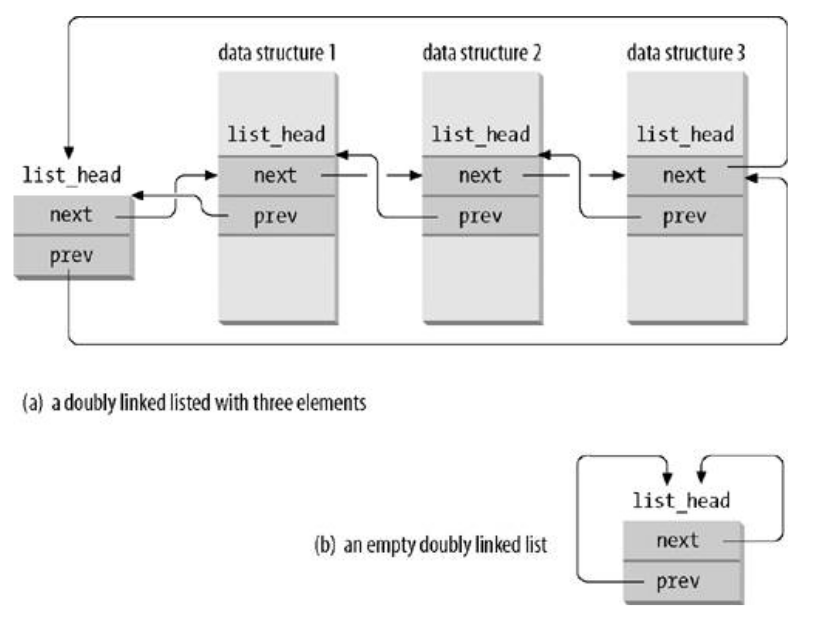
\includegraphics[width=1.0\textwidth]{listhead.png}
\end{frame}

\begin{frame}[fragile]
\frametitle{用list\_head实现双向链表: 关键问题}
\begin{block}{include/linux/list.h}
\lstlisthead
\end{block}
\begin{block}{include/linux/sched.h}
\lstlistheadusage
\end{block}
\begin{block}{关键问题}
如何根据list\_head的地址确定包含它的数据结构的地址?
\end{block}
\end{frame}

\begin{frame}[fragile]
\frametitle{如何计算包含list\_head的结构体地址?}
\begin{block}{宏list\_entry(ptr, type, member)}
计算包含ptr(指向list\_head结构的指针)的结构体的地址
\end{block}
\begin{block}{例子: 结合上述task\_struct结构}
list\_entry(ptr, struct task\_struct, run\_list)
\end{block}

\begin{block}{思考}
宏list\_entry的实现原理是什么?
\end{block}

\end{frame}

%\defverbatim[colored]\lstcontainerof{
%\begin{lstlisting}[tabsize=8,basicstyle=\ttfamily]
%#define container_of(ptr, type, member) ({  \
%const typeof( ((type *)0)->member ) *__mptr = (ptr);\
%(type *)( (char *)__mptr - offsetof(type,member) );})
%\end{lstlisting}
%}
\defverbatim[colored]\lstcontainerof{
\begin{lstlisting}[tabsize=8,basicstyle=\ttfamily]
#define list_entry(ptr, type, member) \
    container_of(ptr, type, member)
\end{lstlisting}
}
\begin{frame}[fragile]
\frametitle{如何计算包含list\_head的结构体地址?}
\begin{block}{include/linux/list.h}
\lstcontainerof
\end{block}
\begin{block}{container\_of的定义}
请在include/linux/kernel.h中找到container\_of的定义并试着理解它。
\end{block}
\end{frame}


\defverbatim[colored]\lstinit{
\begin{lstlisting}[tabsize=8,basicstyle=\ttfamily]
#define LIST_HEAD_INIT(name) \
        { &(name), &(name) }

#define LIST_HEAD(name) \
    struct list_head name = LIST_HEAD_INIT(name)
\end{lstlisting}
}
\begin{frame}[fragile]
\frametitle{list\_head结构的静态初始化}
\begin{block}{include/linux/list.h}
\lstinit
\end{block}
\begin{block}{LIST\_HEAD的使用方法}
%\lstinit
例: \verb|LIST_HEAD(packet_list)|声明一个名为\verb|packet_list|的表头变量并将其初始化为空表。
\end{block}
\end{frame}

\begin{frame}[fragile]
\frametitle{针对list结构的操作}
\begin{itemize}
\item \verb|list_add(new, head)| 把new插入head后面
\item \verb|list_add_tail(new, head)| 把new插入head前面
\item \verb|list_del(entry)| 把entry从链表中删除
\item \verb|list_empty(head)| 判断链表head是否为空
\item \verb|list_splice(list, head)| 合并list和head
\item \verb|list_for_each(pos, head)| 遍历以head为头的链表
\item \verb|list_for_each_entry(pos, head)|
\end{itemize}
\end{frame}

\defverbatim[colored]\lstadd{
\begin{lstlisting}[tabsize=8,basicstyle=\ttfamily]
typedef struct list_head list_head;

static inline void list_add(list_head *new, 
                            list_head *head)
{
    __list_add(new, head, head->next);
}

static inline void __list_add(list_head *new,
                  list_head *prev,
                  list_head *next)
{
    next->prev = new;
    new->next  = next;
    new->prev  = prev;
    prev->next = new;
}
\end{lstlisting}
}
\begin{frame}[fragile]
\frametitle{针对list结构的操作举例: list\_add}
\lstadd
\end{frame}

\defverbatim[colored]\lstforeach{
\begin{lstlisting}[tabsize=8,basicstyle=\ttfamily]
struct list_head *p;

list_for_each(p, &list) {
    if (!condition) continue;
    return list_entry(p, struct task_struct, 
                      run_list);
}

return NULL;
\end{lstlisting}
}
\begin{frame}[fragile]
\frametitle{针对list结构的操作举例: list\_for\_each}
\lstforeach
\end{frame}

\begin{frame}[fragile]
\frametitle{针对list结构的操作: 其它}
\begin{block}{课外练习}
从源文件include/linux/list.h中找出上述list操作的函数代码,阅读并理解其实现。
\end{block}
\end{frame}

\subsection{哈希表: hlist\_head与hlist\_node}

\defverbatim[colored]\lsthlist{
\begin{lstlisting}[tabsize=8,basicstyle=\ttfamily]
struct hlist_head {
    struct hlist_node *first;
};

struct hlist_node {
    struct hlist_node *next, **pprev;
};
\end{lstlisting}
}
\begin{frame}[fragile]
\frametitle{实现哈希表: hlist\_head与hlist\_node}
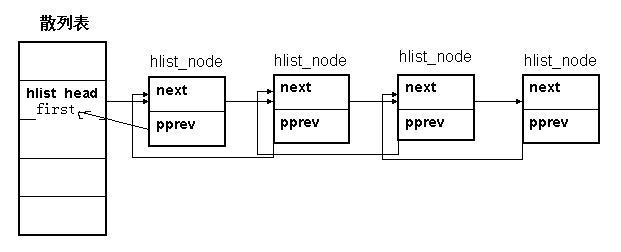
\includegraphics[width=0.9\textwidth]{hlist.jpeg}
\begin{block}{include/linux/list.h}
\lsthlist
\end{block}
\end{frame}

\begin{frame}[fragile]
\frametitle{针对hlist\_head与hlist\_node的操作}
\begin{itemize}
\item \verb|hlist_add_head|
\item \verb|hlist_add_before|
\item \verb|hlist_del(entry)|
\item \verb|hlist_empty(head)| 
\item \verb|hlist_entry(head)| 
\item \verb|hlist_for_each_entry(pos, head)|
\end{itemize}
\end{frame}

\begin{frame}[fragile]
\frametitle{Linux内核关键数据结构:hlist\_head与hlist\_node}
\begin{block}{思考及课外练习}
阅读include/linux/list.h中
\verb|hlist_add_head()|, \verb|hlist_del()|, \verb|hlist_empty()|, \verb|hlist_add_before()|等函数的实现,思考:

\begin{enumerate}
\item \verb|hlist_node|中的\verb|pprev|字段指向什么内容?
\item 为什么\verb|pprev|采用二重指针?
\item 为什么\verb|hlist_head|中只有一个成员\verb|first|?
\item \verb|hlist_head|可否直接用\verb|hlist_node|代替?
\end{enumerate}
\end{block}
\end{frame}

\defverbatim[colored]\lstaddbefore{
\begin{lstlisting}[tabsize=8,basicstyle=\ttfamily]
static inline void hlist_add_before(
                   struct hlist_node *n,
                   struct hlist_node *next)
{
    n->pprev = next->pprev;
    n->next = next;
    next->pprev = &n->next;
    *(n->pprev) = n;
}
\end{lstlisting}
}
\begin{frame}[fragile]
\frametitle{实现哈希表: hlist\_head与hlist\_node}
\begin{block}{include/linux/list.h}
\lstaddbefore
\end{block}
要理解这其中四条语句特别是最后一条的含义。
\end{frame}


\section{Linux进程描述符task\_struct}

\subsection{进程控制块, 进程描述符}

\begin{frame}{进程控制块(PCB)}
\begin{columns}%[t]
\column{.5\textwidth}
用于存放与每个进程相关的信息
\begin{itemize}
\item 进程状态
\item 程序计数器PC
\item CPU寄存器
\item CPU调度信息
\item 内存管理信息
\item I/O状态信息
\item 记账信息
\end{itemize}
\column{.5\textwidth}
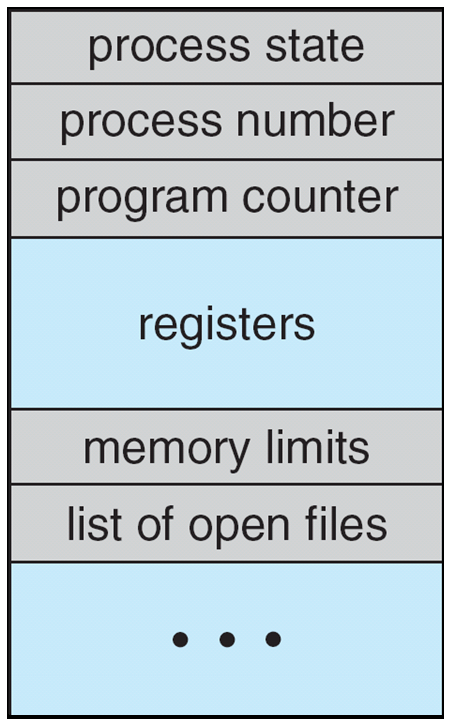
\includegraphics[width=0.6\textwidth]{PCB.png}
\end{columns}%[t]
\end{frame}

\begin{frame}{Linux进程描述符}
\begin{itemize}
\item 进程控制块在Linux内核中被成为进程描述符(Process Descriptor)
\item 结构名字: struct task\_struct;
\item 这是一个非常大的数据结构,其中包含:
\begin{itemize}
\item 94行成员字段
\item 其中36行成员本身又是struct或者指向struct的指针
\end{itemize}
\item 后面我们将对task\_struct结构进行逐行分析
\end{itemize}
\end{frame}

\begin{frame}{Linux进程描述符}
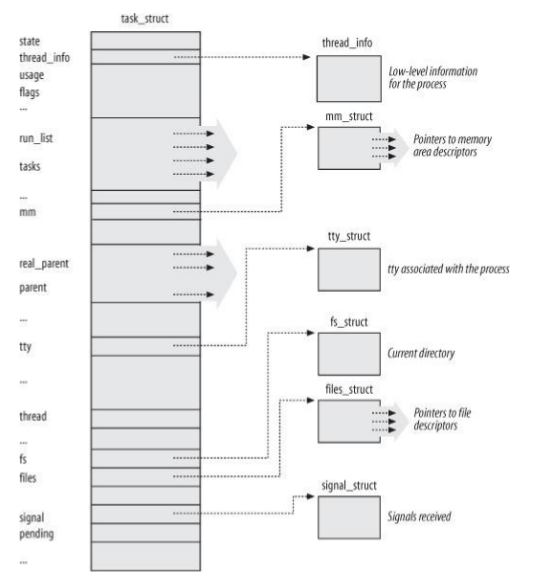
\includegraphics[width=0.7\textwidth]{taskstruct.png}
\end{frame}

\subsection{进程描述符各字段分析}

\defverbatim[colored]\lstpidmax{
\begin{lstlisting}[tabsize=8,basicstyle=\ttfamily]
/*
 * This controls the default maximum pid 
 *   allocated to a process
 */
#define PID_MAX_DEFAULT 0x8000
\end{lstlisting}
}
\begin{frame}{Linux区别进程的方式: pid字段}
%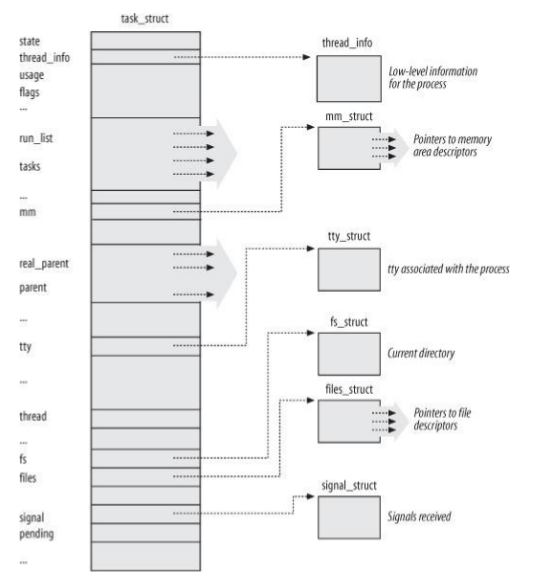
\includegraphics[width=0.7\textwidth]{taskstruct.png}
\begin{itemize}
\item 在内核中,对进程的各种操作均通过task\_struct实现
\item 用户角度,每个进程有唯一编号(PID). 进程的PID保存于task\_struct的pid字段中。
\begin{itemize}
\item 例如:kill()系统调用的参数为PID
\item 内核需要快速从PID找到对应的task\_struct进行操作(后面讲具体方法)
\end{itemize}
\end{itemize}
\begin{block}{PID可取的最大值: include/linux/threads.h}
\lstpidmax
\end{block}
\end{frame}

\begin{frame}{Linux区别进程的方式: pid字段}
\begin{block}{思考}
\begin{enumerate}
\item 为什么要限制PID可取的最大值?
\item[]
\item 如果系统中进程个数超过这个最大值怎么办?
\end{enumerate}
\end{block}
\end{frame}

\defverbatim[colored]\lstpidmaparray{
\begin{lstlisting}[tabsize=8,basicstyle=\ttfamily]
typedef struct pidmap {
    atomic_t nr_free;
    void *page;
} pidmap_t;

static pidmap_t pidmap_array[PIDMAP_ENTRIES] =
     { [ 0 ... PIDMAP_ENTRIES-1 ] = 
       { ATOMIC_INIT(BITS_PER_PAGE), NULL } };
\end{lstlisting}
}
\begin{frame}[fragile]
\frametitle{Linux区别进程的方式: pid字段}
\begin{block}{pidmap\_array用于管理pid值的回收利用: kernel/pid.c}
\lstpidmaparray
\end{block}
\begin{block}{思考}
\verb|pidmap_array|的必要性? (从pid分配的角度考虑)
\end{block}
\end{frame}

\defverbatim[colored]\lsttasks{
\begin{lstlisting}[tabsize=8,basicstyle=\ttfamily]
struct task_struct {
    ...
    struct list_head tasks;
    ...
};
\end{lstlisting}
}

\begin{frame}{内核遍历所有进程的方式: tasks字段}
OS有时需要遍历系统中全部进程,所以进程描述符中需要相应字段,用于连接系统中的各个进程。
\begin{itemize}
\item 这就用到前面所说的list\_head这个关键结构
\item 回想一下list\_head中包含的两个字段
\end{itemize}
\end{frame}

\begin{frame}{内核遍历所有进程的方式: tasks字段}
\begin{block}{task\_struct中的tasks字段:将系统中所有进程连接起来} 
\lsttasks
\end{block}
\begin{block}{系统中所有进程组成的链表}
%\lststates
以init\_task为表头,进程描述符的tasks字段将所有进程连接起来
\end{block}
\begin{block}{遍历系统中所有进程的宏: for\_each\_process}
阅读并理解include/linux/sched.h中for\_each\_process的实现。
\end{block}
\end{frame}

\begin{frame}[fragile]
\frametitle{与进程调度相关的字段}
在进程调度时,需要从处于\verb|TASK_RUNNING|(可运行)状态的进程中选择一个,让它占有CPU并运行。
\begin{block}{2.6.x之前的Linux内核}
将所有处于\verb|TASK_RUNNING|状态的进程放到一个链表,需要遍历整个链表,从中选择优先级最高的进程。
调度的时间复杂度为$O(n)$.
\end{block}
\begin{block}{Linux 2.6.x内核的$O(1)$调度算法}
\begin{itemize}
\item 在进程描述符中记录每个进程的优先级
\item 以有效的数据结构按照优先级组织所有进程
\item 调度算法时间复杂度为$O(1)$, 与进程数$n$没有直接关系
\end{itemize}
\end{block}
\end{frame}

\defverbatim[colored]\lstrunning{
\begin{lstlisting}[tabsize=8,basicstyle=\ttfamily]
struct task_struct {
    ...
    int prio, static_prio;
    struct list_head run_list;
    prio_array_t *array;
    ...
};
\end{lstlisting}
}
\begin{frame}%{Linux进程描述符: Process Descriptor}
\frametitle{与进程调度相关的字段}
\lstrunning
\begin{block}{各字段的含义}
\begin{itemize}
\item prio 为进程当前优先级 (0 -- 139)
\item run\_list 用于连接所有相同优先级的进程
\item array?
\end{itemize}
\end{block}
\end{frame}

\defverbatim[colored]\lstprio{
\begin{lstlisting}[tabsize=8,basicstyle=\ttfamily]
struct prio_array {
    unsigned int nr_active;
    unsigned long bitmap[BITMAP_SIZE];
    struct list_head queue[MAX_PRIO];
};
\end{lstlisting}
}
\defverbatim[colored]\lstprioarrayt{
\begin{lstlisting}[tabsize=8,basicstyle=\ttfamily]
typedef struct prio_array prio_array_t;
\end{lstlisting}
}
\begin{frame}%{Linux进程描述符: Process Descriptor}
\frametitle{与进程调度相关的字段}
\begin{block}{kernel/sched.c}
\lstprio
\end{block}
\begin{block}{include/linux/sched.h}
\lstprioarrayt
\end{block}
\begin{block}{各成员字段的含义}
\begin{itemize}
\item nr\_active: 当前列表中进程总数
\item bitmap 用于记录哪个队列为非空(后面分析调度算法时用到)
\item queue用于存储140个队列的表头
\end{itemize}
\end{block}
\end{frame}

\defverbatim[colored]\lstenqueue{
\begin{lstlisting}[tabsize=8,basicstyle=\ttfamily]
void enqueue_task(struct task_struct *p, 
                  prio_array_t *array)
{
    sched_info_queued(p);
    list_add_tail(&p->run_list, 
                  array->queue[p->prio]);
    __set_bit(p->prio, array->bitmap);
    array->nr_active++;
    p->array = array;
}
\end{lstlisting}
}
\begin{frame}{fragile}
\frametitle{与进程调度相关的字段}
\lstenqueue
\begin{block}{特别注意}
list\_add\_tail的第一个参数.
\end{block}

\end{frame}

\begin{frame}[fragile]
\frametitle{课外练习}
\begin{enumerate}
\item 上页中,\verb|BITMAP_SIZE|和\verb|MAX_PRIO|两个宏分别在文件kernel/sched.c和include/linux/sched.h中定义,
请确定这两个宏的具体数值。
\item[]
\item 在文件kernel/sched.c找出\verb|dequeue_task|的定义并理解它。
\end{enumerate}
\end{frame}

\begin{frame}{表示进程状态的字段: state}
\begin{block}{include/linux/sched.h}
\lstPCBstate
\end{block}
\begin{block}{进程可能的状态: include/linux/sched.h}
\lststates
\end{block}
\end{frame}

\begin{frame}[fragile]
\frametitle{表示进程状态的字段: state}
\begin{block}{改变进程状态的函数/宏}
\begin{itemize}
\item \verb|set_task_state| 改变指定进程的状态
\item \verb|set_current_state| 改变当前执行的进程的状态
\end{itemize}
\end{block}
\begin{block}{课外练习}
阅读以上两个函数的源代码(位于文件include/linux/sched.h),并思考为什么要这样写。
\end{block}
\end{frame}

%\begin{frame}[fragile]%{Linux内核关键数据结构:list}
%\frametitle{Linux中的内核地址空间与用户地址空间}
%\begin{columns}%[b]
%\column{.4\textwidth}
%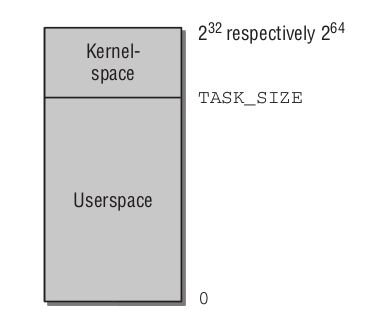
\includegraphics[width=1.0\textwidth]{as.png}
%\column{.6\textwidth}
%\begin{itemize}
%\item 用户地址空间从0到TASK\_SIZE-1
%\item 内核地址空间从TASK\_SIZE到$2^{32}$-1
%\end{itemize}
%\end{columns}
%\end{frame}
%
%\begin{frame}[fragile]%{Linux内核关键数据结构:list}
%\frametitle{Linux中的内核地址空间与用户地址空间}
%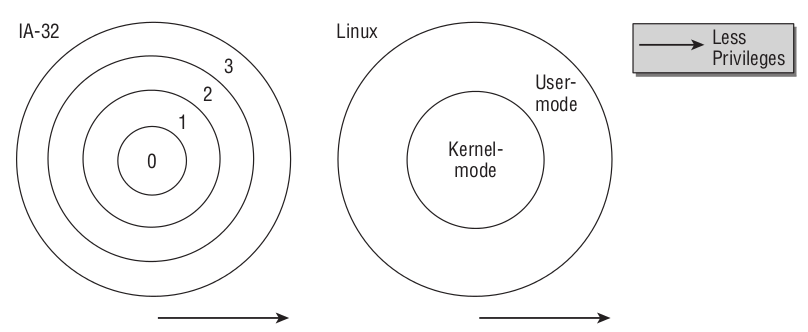
\includegraphics[width=1.0\textwidth]{ring.png}
%\begin{itemize}
%\item 用户态下只能访问用户地址空间
%\item 核心态下可以访问所有地址空间
%\item 二者其他区别?
%\end{itemize}
%\end{frame}

%\begin{frame}[fragile]%{Linux内核关键数据结构:list}
%\frametitle{分页技术与地址空间共享}
%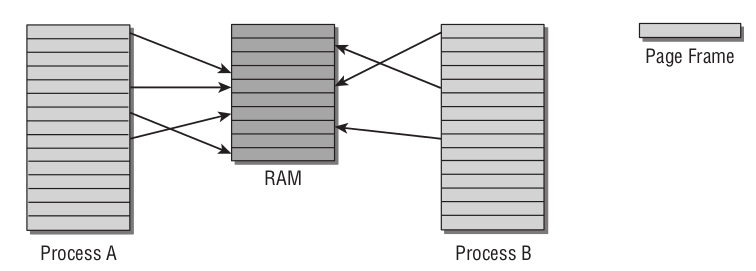
\includegraphics[width=1.0\textwidth]{paging.png}
%
%注意观察A、B进程的第0页面对应的物理页框;地址空间的共享(代码、数据)
%\end{frame}

%\begin{frame}[fragile]%{Linux内核关键数据结构:list}
%\frametitle{Linux下的多级分页技术}
%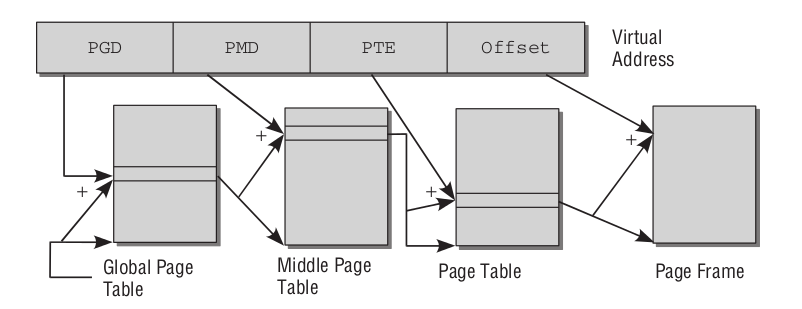
\includegraphics[width=1.0\textwidth]{pagetables.png}
%
%CPU内部进行地址映射的两个硬件单元:MMU/TLB
%\end{frame}

%\begin{frame}[fragile]%{Linux内核关键数据结构:list}
%\frametitle{物理内存的分配算法:伙伴系统}
%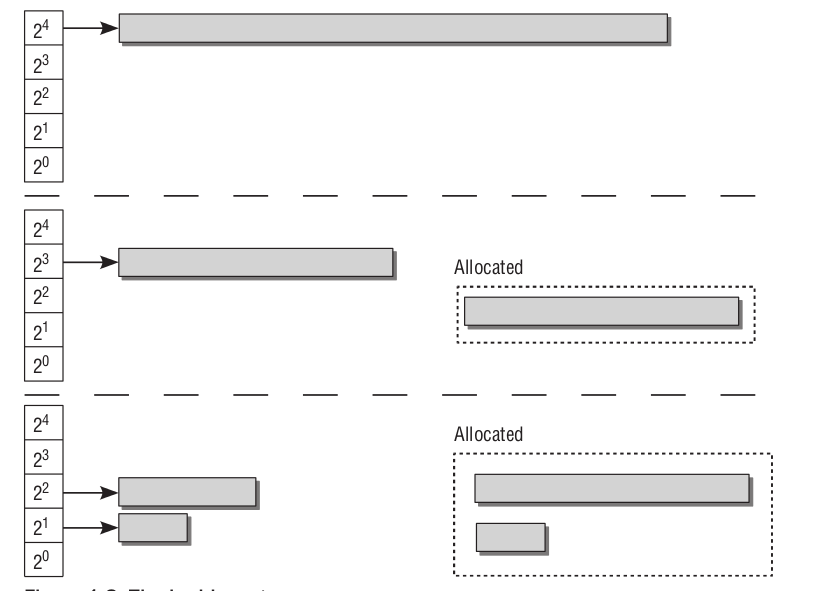
\includegraphics[width=0.8\textwidth]{buddy.png}

%注意观察A、B进程的第0页面对应的物理页框;地址空间的共享(代码、数据)
%\end{frame}


\defverbatim[colored]\lstparents{
\begin{lstlisting}[tabsize=8,basicstyle=\ttfamily]
struct task_struct {
    ...
    struct task_struct *real_parent; 
    struct task_struct *parent; 
    struct list_head children; 
    struct list_head sibling; 
    ...
};
\end{lstlisting}
}
\begin{frame}[fragile]
\frametitle{记录进程之间层次关系的字段}
进程管理中需要记录进程之间的层次关系(父母、兄弟姐妹).

\lstparents
\end{frame}

\begin{frame}[fragile]
\frametitle{记录进程之间层次关系的字段}
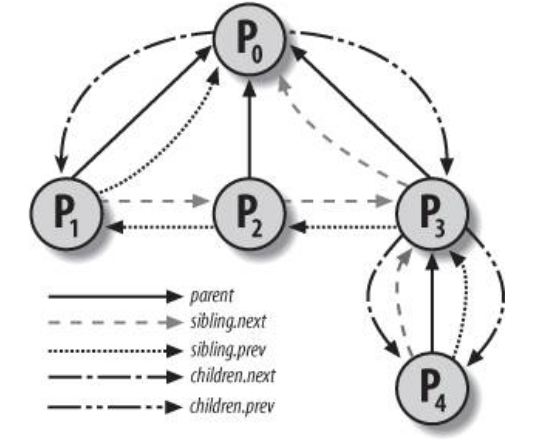
\includegraphics[width=0.8\textwidth]{parent2.png}
\end{frame}

\begin{frame}[fragile]
\frametitle{记录进程之间层次关系的字段}
查看进程结构树的命令:pstree
\end{frame}

\begin{frame}[fragile]
\frametitle{表示进程其他关系的字段}
除了上述关系外,进程之间还存在如下关系:
\begin{itemize}
\item 多个进程可以形成一个组(group),每个组都有唯一的leader.
\begin{itemize}
\item 例如: \verb=cat file | grep 'abc' | wc -l=,其中三个进程形成一个组
\end{itemize}
\item 类似,进程间可以形成一个会话(session),每个会话中指定唯一的leader
\item 同一进程创建的多个线程组成线程组(thread group),每组也有唯一leader
\begin{itemize}
\item 线程组对应多线程程序里的所有线程
\end{itemize}
\end{itemize}
\end{frame}

\defverbatim[colored]\lstotherrelations{
\begin{lstlisting}[tabsize=8,basicstyle=\ttfamily]
struct task_struct {
    ...
    struct task_struct *group_leader;
    pid_t tgid;
    pid_t pid;
    struct signal_struct *signal;
    ...
};
\end{lstlisting}
}
\begin{frame}[fragile]
\frametitle{表示进程其他关系的字段}
task\_struct中的group\_leader和tgid分别表示该进程所在的进程组的leader、线程组的leader:

\lstotherrelations
\end{frame}

\defverbatim[colored]\lstsignalstruct{
\begin{lstlisting}[tabsize=8,basicstyle=\ttfamily]
struct signal_struct {
    ...
    /* job control IDs */
    pid_t pgrp;
    pid_t session;
    ...
};
\end{lstlisting}
}
\begin{frame}[fragile]
\frametitle{表示进程其他关系的字段}
pgrp和session字段分别表示进程组leader的PID、会话组leader的PID:
\begin{block}{include/linux/sched.h}
\lstsignalstruct
\end{block}
\end{frame}

\begin{frame}[fragile]
%\frametitle{Linux进程表示:task\_struct结构}
\frametitle{表示进程其他关系的字段}
进程标识:

\begin{itemize}
\item 从内核角度,一律通过task\_struct操作进程
\item 从用户角度可能需要通过PID操作进程,如kill(pid)
\end{itemize}

所以需要做到从pid到task\_struct的快速转换:

\begin{itemize}
\item task\_struct到pid: \verb|p->pid|
\item pid到task\_struct的快速转换:
\begin{itemize}
\item 遍历所有进程,逐一检查其pid字段的值?
\item 通过散列表结构做到快速转换
\end{itemize}
\item (重要)给定进程组、会话组或者线程组的leader ID, 如何快速找出该组中所有进程(线程)?
\end{itemize}

\end{frame}

\defverbatim[colored]\lstpidtype{
\begin{lstlisting}[tabsize=8,basicstyle=\ttfamily]
enum pid_type
{
    PIDTYPE_PID,
    PIDTYPE_TGID,
    PIDTYPE_PGID,
    PIDTYPE_SID,
    PIDTYPE_MAX
};
\end{lstlisting}
}
\defverbatim[colored]\lstpidhashhaha{
\begin{lstlisting}[tabsize=8,basicstyle=\ttfamily]
static struct hlist_head *pid_hash[PIDTYPE_MAX];
\end{lstlisting}
}
\begin{frame}[fragile]
%\frametitle{Linux进程表示:task\_struct结构}
\frametitle{表示进程其他关系的字段}
共有四种类型的PID:进程本身PID、线程组leader的PID、进程组leader的PID以及会话组leader的PID:
\begin{block}{include/linux/pid.h}
\lstpidtype
\end{block}
\begin{block}{依据PID类型不同,共定义四个散列表:kernel/pid.c}
\lstpidhashhaha
\end{block}
%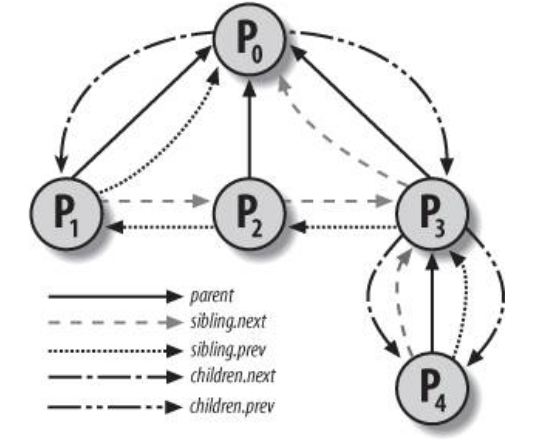
\includegraphics[width=0.8\textwidth]{parent2.png}
\end{frame}

\defverbatim[colored]\lstpidstruct{
\begin{lstlisting}[tabsize=8,basicstyle=\ttfamily]
struct pid
{
    int nr;
    struct hlist_node pid_chain;
    struct list_head pid_list;
};
\end{lstlisting}
}
\defverbatim[colored]\lstpidsintaskstruct{
\begin{lstlisting}[tabsize=8,basicstyle=\ttfamily]
struct task_struct
{
    ...
    /* PID/PID hash table linkage. */
    struct pid pids[PIDTYPE_MAX];
    ...
};
\end{lstlisting}
}
\begin{frame}[fragile]
\frametitle{表示进程其他关系的字段}
\begin{block}{散列表中元素struct pid: include/linux/pid.h }
\lstpidstruct
\end{block}
\begin{block}{task\_struct中相应字段}
\lstpidsintaskstruct
\end{block}
\end{frame}

\defverbatim[colored]\lsthashfunction{
\begin{lstlisting}[tabsize=8,basicstyle=\ttfamily]
unsigned long hash_long(unsigned long val, unsigned int bits)
{
    unsigned long hash = val * 0x9e370001UL;
    return hash >> (32 - bits);
}
\end{lstlisting}
}
\begin{frame}[fragile]
\frametitle{表示进程其他关系的字段}
\begin{block}{哈希函数的定义}
\lsthashfunction
\end{block}
\end{frame}

\begin{frame}[fragile]
\frametitle{表示进程其他关系的字段: 简单哈希表示意图}
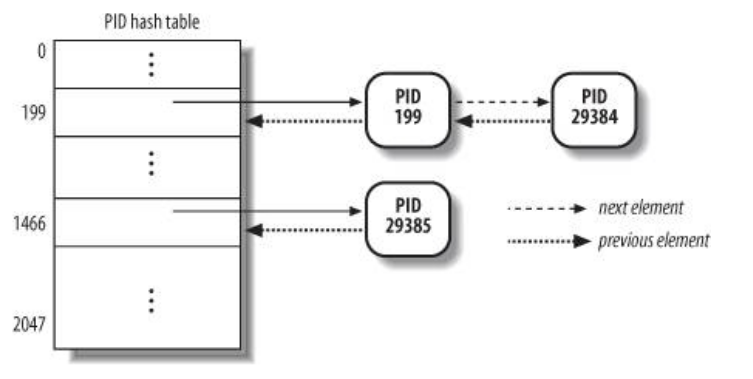
\includegraphics[width=0.8\textwidth]{pidhash.png}
\end{frame}

\begin{frame}[fragile]
\frametitle{表示进程其他关系的字段: pid\_hash结构图} 
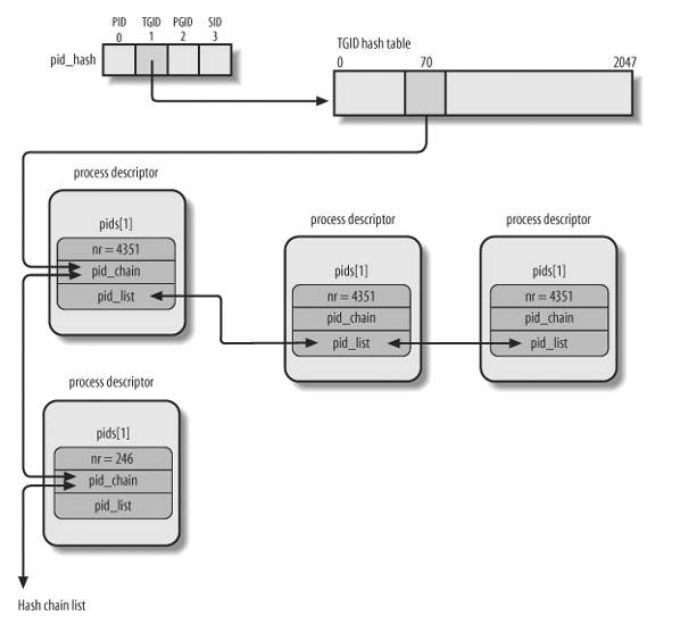
\includegraphics[width=0.8\textwidth]{pidhashes.png}
\end{frame}

\begin{frame}[fragile]
\frametitle{处于等待态的进程如何组织}
\begin{block}{Linux中等待态进程的表示}
\begin{itemize}
\item \verb|TASK_INTERRUPTIBLE|
\item \verb|TASK_UNINTERRUPTIBLE|
\end{itemize}
\end{block}
\begin{block}{进入等待态的原因(所要等待的事件)}
\begin{itemize}
\item 等待磁盘操作结束
\item 等待固定时间(如1秒)
\item 等待互斥锁的释放
\item 等待其他临界资源
\item ...
\end{itemize}
\end{block}
\end{frame}

\defverbatim[colored]\lstwaitqueuehead{
\begin{lstlisting}[tabsize=8,basicstyle=\ttfamily]
struct __wait_queue_head {
    spinlock_t lock;
    struct list_head task_list;
};
\end{lstlisting}
}
\begin{frame}[fragile]
\frametitle{处于等待态的进程如何组织: 等待队列}
\begin{block}{等待队列(wait queue)}
把等待同一事件的进程放到一个等待队列中去。一旦所等待的事件发生,则可以唤醒该队列中的进程。
\end{block}
\begin{block}{wait queue表头的定义: include/linux/wait.h}
\lstwaitqueuehead
\end{block}
其中,字段\verb|lock|用来实现对等待队列的互斥访问(因为内核中有多个地方可能需要对该队列进程操作)。
\end{frame}


\defverbatim[colored]\lstwaitqueue{
\begin{lstlisting}[tabsize=8,basicstyle=\ttfamily]
struct __wait_queue {
    unsigned int flags;
    struct task_struct * task;
    wait_queue_func_t func;
    struct list_head task_list;
};
\end{lstlisting}
}
\begin{frame}[fragile]
\frametitle{处于等待态的进程如何组织: 等待队列中的元素}
\begin{block}{include/linux/wait.h}
\lstwaitqueue
\end{block}
\begin{itemize}
\item flags表示该进程等待的事件是否为exclusive
\item task为进入等待队列的进程
\item func为唤醒该进程的方式(函数)
\item task\_list用于将所有进程连接成队列
\end{itemize}
\end{frame}

\begin{frame}[fragile]
\frametitle{处于等待态的进程如何组织}
\begin{block}{exlusive进程和non-exlusive进程}
\begin{itemize}
\item exlusive进程: 该进程等待的资源不能共享, flags设为1
\begin{itemize}
\item 例如该进程等待的是进入临界区的机会
\end{itemize}
\item non-exclusive进程: 该进程等待的事件/资源可以共享, flags设为0
\begin{itemize}
\item 例如该进程等待的是磁盘数据传输
\end{itemize}
\end{itemize}
\end{block}
\begin{block}{思考}
为什么将flags放到\verb|__wait_queue|而不是放到\verb|__wait_queue_head|中去?
\end{block}
\end{frame}

\begin{frame}[fragile]
\frametitle{对等待队列(wait queue)的操作: 初始化}
\begin{block}{include/linux/wait.h}
\begin{itemize}
\item \verb|DECLARE_WAIT_QUEUE_HEAD(name)|声明名为name的队头并初始化
\item \verb|init_waitqueue_head(q)| 对动态分配的队头q初始化
\item \verb|init_waitqueue_entry(p,q)|对队列元素q初始化:
\begin{verbatim}
q->flags = 0;
q->task = p;
q->func = default_wake_function;
\end{verbatim}
\item \verb|DEFINE_WAIT(name)|将当前占有CPU的进程封装为名为name的队列元素
\end{itemize}
\end{block}
\begin{block}{课外练习}
阅读并理解上述对队列头和队列元素初始化的函数或者宏。
\end{block}
\end{frame}

\begin{frame}[fragile]
\frametitle{对等待队列的操作: 队列元素的插入和删除}
\begin{block}{kernel/wait.c}
\begin{itemize}
\item \verb|add_wait_queue(q, wait)|
\item \verb|add_wait_queue_exclusive(q, wait)|
\item \verb|remove_wait_queue(q, wait)|
\item \verb|waitqueue_active(q)| 功能是什么?(include/linux/wait.h)
\end{itemize}
\end{block}
\end{frame}

\begin{frame}[fragile]
\frametitle{对等待队列的操作: 进程如何将自己放入等待队列?}
\begin{itemize}
\item \verb|sleep_on|
\item \verb|interruptible_sleep_on|
\item \verb|sleep_on_timeout|
\item \verb|interruptible_sleep_on_timeout|
\end{itemize}
\end{frame}

\defverbatim[colored]\lstsleepon{
\begin{lstlisting}[tabsize=8,basicstyle=\ttfamily]
void sleep_on(wait_queue_head_t *wq)
{
    wait_queue_t wait;
    init_waitqueue_entry(&wait, current);
    current->state = TASK_UNINTERRUPTIBLE;
    add_wait_queue(wq, &wait);
    schedule();
    remove_wait_queue(wq, &wait);
}
\end{lstlisting}
}
\begin{frame}[fragile]
\frametitle{对等待队列的操作: 进程如何将自己放入等待队列?}
\lstsleepon
\end{frame}

\begin{frame}[fragile]
\frametitle{对等待队列的操作: 进程如何将自己放入等待队列?}
%\lstsleepon
\begin{itemize}
\item \verb|prepare_to_wait|
\item \verb|prepare_to_wait_exclusive|
\item \verb|finish_wait|
\end{itemize}
\end{frame}

\defverbatim[colored]\lstspreparetowait{
\begin{lstlisting}[tabsize=8,basicstyle=\ttfamily]
DEFINE_WAIT(wait);
prepare_to_wait(&wq,&wait,TASK_INTERRUPTIBLE);
...
if (!condition)
    schedule();
finish_wait(&wq, &wait);
\end{lstlisting}
}
\begin{frame}[fragile]
\frametitle{对等待队列的操作: 进程如何将自己放入等待队列?}
\lstspreparetowait
\end{frame}

\defverbatim[colored]\lstwaitevent{
\begin{lstlisting}[tabsize=8,basicstyle=\ttfamily]
DEFINE_WAIT(wait);
for (;;) {
    prepare_to_wait(&wq, &wait,
                    TASK_UNINTERRUPTIBLE);
    if (condition)
        break;
    schedule();
}
finish_wait(&wq, &wait);
\end{lstlisting}
}
\begin{frame}[fragile]
\frametitle{对等待队列的操作: wait\_event(condtion)}
\lstwaitevent
\end{frame}

\begin{frame}[fragile]
\frametitle{对等待队列的操作: 如何把队列中的进程唤醒?}
%\lstwaitevent
\begin{itemize}
\item \verb|wake_up|
\item \verb|wake_up_nr|
\item \verb|wake_up_all|
\item \verb|wake_up_interruptible|
\item \verb|wake_up_interruptible_nr|
\item \verb|wake_up_interruptible_all|
\item \verb|wake_up_interruptible_sync|
\item \verb|wake_up_locked|
\end{itemize}
\end{frame}

\begin{frame}[fragile]
\frametitle{对等待队列的操作: 如何把队列中的进程唤醒?}
\begin{itemize}
\item 所有non-exclusive的进程都被唤醒
\item 如果名字中没有interruptible, 则唤醒所有睡眠进程(\verb|TASK_INTERRUPTIBLE|及\verb|TASK_UNINTERRUPTIBLE|).
否则,只唤醒队列中\verb|TASK_INTERRUPTIBLE|状态的进程。
\item 名字中含有nr的宏唤醒指定个数的exclusive进程
\item 名字中含有all的宏唤醒全部指定状态的exclusive进程
\item 名字中没有nr或者all的宏只唤醒一个exclusive进程
\end{itemize}
\end{frame}

\defverbatim[colored]\lstwakeupimple{
\begin{lstlisting}[tabsize=8,basicstyle=\ttfamily]
void wake_up(wait_queue_head_t *q)
{
    struct list_head *tmp;
    wait_queue_t *curr;

    list_for_each(tmp, &q->task_list) {
        curr = list_entry(tmp, wait_queue_t, task_list);
        if (curr->func(curr, 
                       TASK_INTERRUPTIBLE|
                       TASK_UNINTERRUPTIBLE, 0, NULL) 
            && curr->flags)
            break;
    }
}
\end{lstlisting}
}
%\begin{frame}[fragile]
%\frametitle{对等待队列的操作: 如何把队列中的进程唤醒?}
%\lstwakeupimple
%\end{frame}

\begin{frame}[fragile]
\frametitle{Linux进程表示:task\_struct结构}
\begin{block}{task\_struct结构的rlim字段: include/linux/resource.h}
\begin{verbatim}
struct rlimit {
    unsigned long   rlim_cur;
    unsigned long   rlim_max;
};

struct task_struct {
    ...
    struct rlimit rlim[RLIM_NLIMITS];
    ...
};
\end{verbatim}
\end{block}
\begin{block}{相关系统调用:}
\begin{verbatim}
int getrlimit(int res, struct rlimit *rlim);
int setrlimit(int res, const struct rlimit *rlim);
\end{verbatim}
\end{block}
\end{frame}

\begin{frame}[fragile]
\frametitle{Linux进程表示:task\_struct结构}
\begin{block}{task\_struct结构的rlim字段: include/asm-generic/resource.h}
\begin{verbatim}
#define RLIMIT_CPU      0   
#define RLIMIT_FSIZE        1  
#define RLIMIT_DATA     2   
#define RLIMIT_STACK        3 
#define RLIMIT_CORE     4   
#define RLIMIT_NOFILE      7  
...
#define RLIM_NLIMITS        15
\end{verbatim}
\end{block}
\begin{block}{相关命令}
cat /proc/self/limits
\end{block}
\end{frame}

\defverbatim[colored]\lstthreadintask{
\begin{lstlisting}[tabsize=8,basicstyle=\ttfamily]
struct task_struct {
    ...
    struct user_struct thread;
    ...
};
\end{lstlisting}
}
\begin{frame}[fragile]
\frametitle{Linux进程表示:task\_struct结构}
\lstthreadintask
\end{frame}

\defverbatim[colored]\lstthreadstruct{
\begin{lstlisting}[tabsize=8,basicstyle=\ttfamily]
struct thread_struct {
    unsigned long   rsp0;
    unsigned long   rsp;
    unsigned long   fs;
    unsigned long   gs;
    unsigned short  es, ds, fsindex, gsindex;
    ...
};
\end{lstlisting}
}
\begin{frame}[fragile]
\frametitle{Linux进程表示:task\_struct结构}
\begin{block}{include/asm-x86\_64/processor.h}
\lstthreadstruct
\end{block}
\begin{block}{通用寄存器的值保存在哪里?}
\alert{eax}, \alert{ebx}等通用寄存器在上下文切换时保存在kernel mode stack (核心态下的栈中)
\end{block}
\end{frame}

%\begin{frame}{名字空间(namespaces)的概念}
%
%传统UNIX只有唯一的名字空间:
%
%\begin{description}
%\item[PID] 进程编号
%\item[UID] 用户编号
%\item[GID] 群组编号
%\end{description}
%
%\begin{block}{唯一名字空间的缺点举例}
%计算服务提供商:希望为用户提供Linux操作系统的使用服务,每个用户都可以拥有root权限。
%\end{block}
%
%\begin{block}{解决方法}
%\begin{itemize}
%\item 每个用户一台机器?
%\item 虚拟机(VMWare)?
%\end{itemize}
%\end{block}
%
%\end{frame}
%
%\begin{frame}{名字空间(namespaces)的概念}
%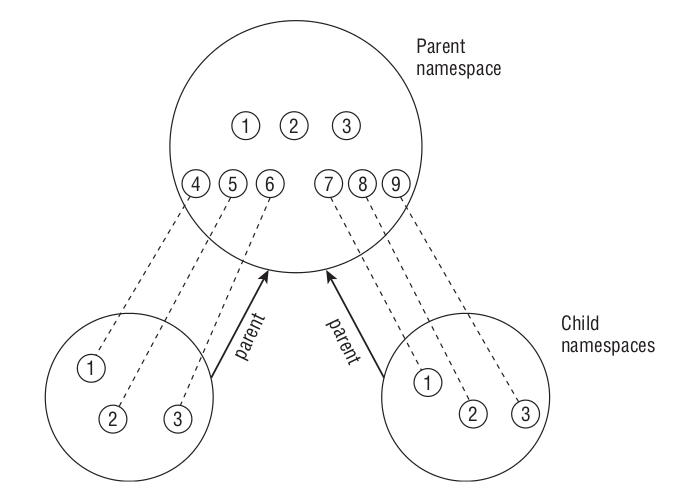
\includegraphics[width=0.9\textwidth]{ns.png}
%\begin{block}{名字空间的相互关系}
%上图中,子名字空间中的1,2,3编号与父名字空间中的1,2,3完全不相关
%\end{block}
%\end{frame}

%\begin{frame}[fragile]
%\frametitle{Linux内核中名字空间的实现}
%\begin{block}{struct nsproxy: 按照功能划分若干名字空间 -- include/linux/nsproxy.h}
%\begin{verbatim}
%struct nsproxy {
%    atomic_t count;
%    struct uts_namespace *uts_ns;
%    struct ipc_namespace *ipc_ns;
%    struct mnt_namespace *mnt_ns;
%    struct pid_namespace *pid_ns;
%    struct user_namespace *user_ns;
%    struct net       *net_ns;
%};
%\end{verbatim}
%\end{block}
%\end{frame}

%\begin{frame}[fragile]
%\frametitle{Linux内核中名字空间的实现}
%%\begin{block}{struct nsproxy: 按照功能划分若干名字空间 -- include/linux/sched.h}
%\begin{verbatim}
%struct task_struct {
%    ...
%    struct nsproxy *nsproxy;
%    ...
%}
%\end{verbatim}
%\end{block}
%\end{frame}

%\begin{frame}{Linux内核中名字空间的实现}
%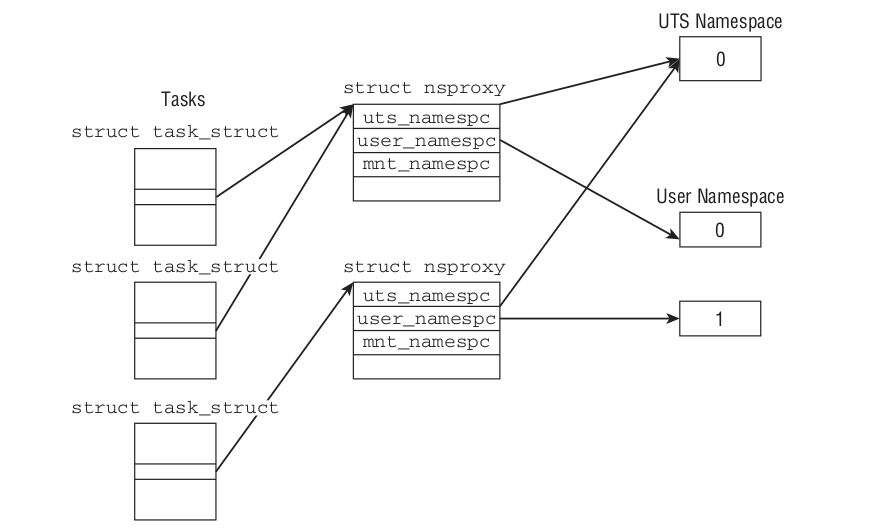
\includegraphics[width=0.9\textwidth]{ns_impl.png}
%\end{frame}

%\begin{frame}[fragile]
%\frametitle{Linux内核中名字空间的实现}
%\begin{block}{fork新进程时可以指明是否为此进程建立新的名字空间:}
%\begin{verbatim}
%#define CLONE_NEWUTS    0x04000000  
%#define CLONE_NEWIPC    0x08000000 
%#define CLONE_NEWUSER   0x10000000
%#define CLONE_NEWPID    0x20000000
%#define CLONE_NEWNET    0x40000000 
%\end{verbatim}
%\end{block}
%\end{frame}

%\begin{frame}[fragile]
%\frametitle{初始全局名字空间的定义}
%\begin{block}{kernel/nsproxy.c}
%\begin{verbatim}
%struct nsproxy init_nsproxy = \
%       INIT_NSPROXY(init_nsproxy);
%\end{verbatim}
%\end{block}
%\begin{block}{include/linux/init\_task.h}
%\begin{verbatim}
%#define INIT_NSPROXY(nsproxy) {                     \
%    .pid_ns     = &init_pid_ns,                 \
%    .count      = ATOMIC_INIT(1),               \
%    .uts_ns     = &init_uts_ns,                 \
%    .mnt_ns     = NULL,                     \
%    INIT_NET_NS(net_ns)                                             \
%    INIT_IPC_NS(ipc_ns)                     \
%    .user_ns    = &init_user_ns,                \
%}
%
%\end{verbatim}
%\end{block}
%\end{frame}

%\begin{frame}[fragile]
%\frametitle{UTS Namespace}
%\begin{block}{include/linux/utsname.h}
%\begin{verbatim}
%struct uts_namespace {
%    struct kref kref;
%    struct new_utsname name;
%};

%struct new_utsname {
%    char sysname[65];
%    char nodename[65];
%    char release[65];
%    char version[65];
%    char machine[65];
%    char domainname[65];
%};
%\end{verbatim}
%\end{block}
%\end{frame}
%\begin{frame}[fragile]
%\frametitle{UTS Namespace的初始值}
%\begin{block}{init/version.c}
%\begin{verbatim}
%struct uts_namespace init_uts_ns = {
%    .kref = {
%        .refcount   = ATOMIC_INIT(2),
%    },
%    .name = {
%        .sysname    = UTS_SYSNAME,
%        .nodename   = UTS_NODENAME,
%        .release    = UTS_RELEASE,
%        .version    = UTS_VERSION,
%        .machine    = UTS_MACHINE,
%        .domainname = UTS_DOMAINNAME,
%    },
%};
%\end{verbatim}
%\end{block}
%\end{frame}

%\begin{frame}[fragile]
%\frametitle{User Namespace}
%\begin{block}{include/linux/user\_namespace.h}
%\begin{verbatim}
%struct user_namespace {
%    struct kref kref;
%    struct hlist_head uidhash_table[UIDHASH_SZ];
%    struct user_struct *root_user;
%};
%\end{verbatim}
%\end{block}
%\end{frame}
%
%\begin{frame}[fragile]
%\frametitle{进程间的相互关系}
%\begin{block}{include/linux/sched.h}
%\begin{verbatim}
%struct task_struct {
%    ...
%    struct list_head children; /* children list */
%    struct list_head sibling; /* parent’s children list */
%    ...
%}
%\end{verbatim}
%\end{block}
%\end{frame}

%\begin{frame}{进程间的相互关系}
%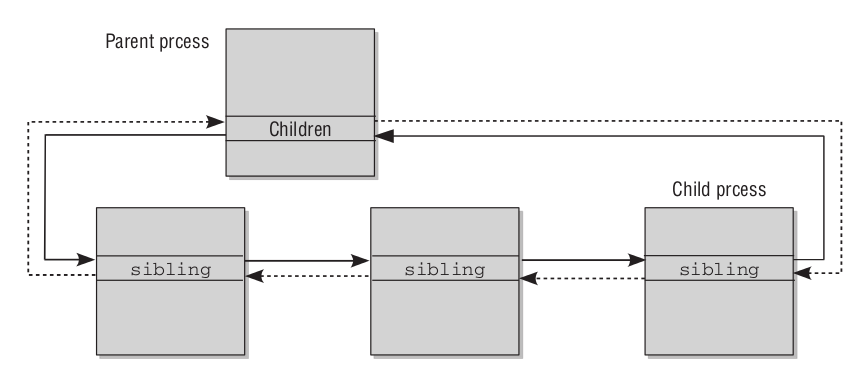
\includegraphics[width=1.0\textwidth]{parent.png}
%\begin{block}{children与sibling}
%\begin{itemize}
%\item children是指向本进程所有子进程的链表表头
%\item sibling用于连接兄弟进程
%\item pstree命令显示进程结构树(用途?)
%\end{itemize}
%\end{block}
%\end{frame}

\begin{frame}{创建进程的系统调用}
\begin{enumerate}
\item fork用于创建新进程
\item[]
\item vfork创建新进程,并且只有当子进程运行完毕,父进程才能运行;二者共享存储空间(deprecated)
\item[]
\item clone用于创建进程或者线程

\end{enumerate}
\end{frame}

\begin{frame}{创建进程的系统调用: 写拷贝技术(copy-on-write)}
历史上,unix中调用fork创建新进程时,OS需要将父进程的存储空间完全拷贝一份给子进程,这有以下缺点:
\begin{itemize}
\item 拷贝内存的过程非常耗时
\item 需要占用大量内存空间
\item 子进程一旦执行exec,则上述拷贝完全浪费
\end{itemize}

写拷贝(copy-on-write): 创建新进程时,仅拷贝父进程的页表,并将所有页表项对应的页面设置成只读,只有当
父亲或子进程需要写入某页面时,才拷贝相应页面的内容。
\end{frame}

\begin{frame}[fragile]
\frametitle{创建进程: do\_fork函数}
\begin{block}{kernel/fork.c}
\begin{verbatim}
long do_fork(unsigned long clone_flags,
             unsigned long stack_start,
             struct pt_regs *regs,
             unsigned long stack_size,
             int __user *parent_tidptr,
             int __user *child_tidptr)
\end{verbatim}
\end{block}
\begin{itemize}
\item clone\_flags用于描述进程的哪些属性将被复制(进程/线程!)
\item start\_stack为用户态下进程的栈起始位置, stack\_size为栈的总长度
\item regs, parent\_tidptr等参数后面讲
\end{itemize}
\end{frame}

\begin{frame}[fragile]
\frametitle{创建进程: do\_fork函数}
\begin{block}{arch/x86/kernel/process\_32.c}
\begin{verbatim}
asmlinkage int sys_fork(struct pt_regs regs)
{
    return do_fork(SIGCHLD, regs.esp, &regs, 
                   0, NULL, NULL);
}
\end{verbatim}
\end{block}
\end{frame}

\begin{frame}[fragile]
\frametitle{创建进程: do\_fork函数}
\begin{block}{arch/x86/kernel/process\_32.c}
\begin{verbatim}
asmlinkage int sys_clone(struct pt_regs regs)
{
    unsigned long clone_flags;
    unsigned long newsp;
    int __user *parent_tidptr, *child_tidptr;
    clone_flags = regs.ebx;
    newsp = regs.ecx;
    parent_tidptr = (int __user *)regs.edx;
    child_tidptr = (int __user *)regs.edi;
    if (!newsp)
        newsp = regs.esp;
    return do_fork(clone_flags, newsp, &regs, 
                   0, parent_tidptr, child_tidptr);
}

\end{verbatim}
\end{block}
\end{frame}

%\begin{frame}[fragile]
%\frametitle{创建进程: do\_fork函数的实现}
%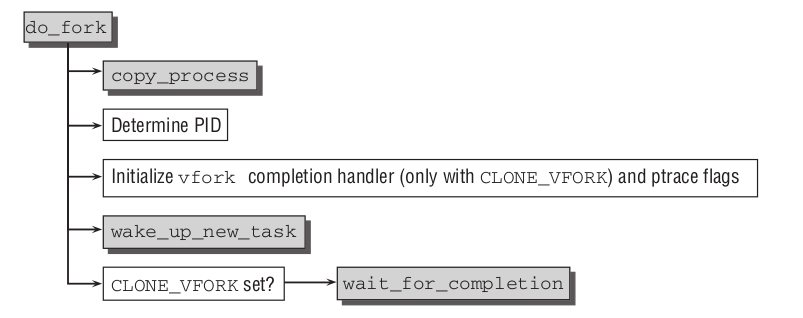
\includegraphics[width=1.0\textwidth]{dofork.png}
%\end{frame}

\end{CJK*}
\end{document}
